\let\negmedspace\undefined
\let\negthickspace\undefined
\documentclass[journal]{IEEEtran}
\usepackage[a5paper, margin=10mm, onecolumn]{geometry}
\usepackage{lmodern} % Ensure lmodern is loaded for pdflatex
 % Include tfrupee package
\setlength{\headheight}{1cm} % Set the height of the header box
\setlength{\headsep}{0mm}     % Set the distance between the header box and the top of the text
\usepackage{enumitem}
\usepackage{gvv-book}
\usepackage{gvv}
\usepackage{cite}
\usepackage{amsmath,amssymb,amsfonts,amsthm}
\usepackage{algorithmic}
\usepackage{graphicx}
\usepackage{textcomp}
\usepackage{xcolor}
\usepackage{txfonts}
\usepackage{listings}
\usepackage{enumitem}
\usepackage{mathtools}
\usepackage{gensymb}
\usepackage{comment}
\usepackage[breaklinks=true]{hyperref}
\usepackage{tkz-euclide} 
\usepackage{listings}
% \usepackage{gvv}                                        
\def\inputGnumericTable{}                                 
\usepackage[latin1]{inputenc}                                
\usepackage{color}                                            
\usepackage{array}                                            
\usepackage{longtable}                                       
\usepackage{calc}                                             
\usepackage{multirow}                                         
\usepackage{hhline}                                           
\usepackage{ifthen}                                           
\usepackage{lscape}
\begin{document}

\bibliographystyle{IEEEtran}
\vspace{3cm}

\title{1-1.7-5}
\author{AI24BTECH11008- Sarvajith
}
% \maketitle
% \newpage
% \bigskip
{\let\newpage\relax\maketitle}

\renewcommand{\thefigure}{\theenumi}
\renewcommand{\thetable}{\theenumi}
\setlength{\intextsep}{10pt} % Space between text and floats
\numberwithin{equation}{enumi}
\numberwithin{figure}{enumi}
\renewcommand{\thetable}{\theenumi}
\textbf{Question: }\\
Find the value of p for which the points A\myvec{-5\\1}, B\myvec{1\\p}, and C\myvec{4\\-2} are colinear?\\
\textbf{Solution: }\\
\renewcommand{\tablename}{TABLE 1}
\begin{table}[h!]    
 \centering
  \begin{tabular}{|c|c|}
\hline
\textbf{lengths} & \textbf{values}\\
\hline
\textbf{BC} & 5.5cm\\
\hline
\textbf{AL} & 5.3cm\\
\hline
\end{tabular}

  \caption{values of the geometrical points in given question}
  \label{tab1-1.2-18-1}
\end{table}
\textbf{Given,}\\
if three points are collinear then their slope should be equal.\\
\begin{align*}
   \text{slope of AB} &= B - A\\
	&=\myvec{1\\p} - \myvec{-5\\1}  \\
        &= \myvec{1 + 5\\p-1}\\
        &= \myvec{6\\p-1}\\
        &= 6\myvec{1\\\frac{p-1}{6}}\\
    \end{align*}
    \begin{align}
        \therefore \text{slope} &= \frac{p-1}{6}. \label{eq 1-1.7-5-1}
    \end{align}
    \begin{align*}
	    \text{slope of BC} &= C - A\\ 
	    &=\myvec{4\\-2} - \myvec{1\\p} \\
         &= \myvec{4-1\\-2-p}\\
         &= \myvec{3\\-2-p}\\
         &= 3\myvec{1\\\frac{-2-p}{3}}\\
    \end{align*}
    \begin{align}
          \therefore \text{slope} &= \frac{-2-p}{3}. \label{eq 1-1.7-5-2}
\end{align}
slope AB = slope of BC\\
\begin{align*}
    \frac{p-1}{6} &= \frac{-p-2}{3}\\
    3\brak{p-1} &= 6\brak{-p-2}\\
    p - 1 &= -2p - 4\\
        p &= -1\\
\end{align*}


\begin{figure}[h!]
\centering
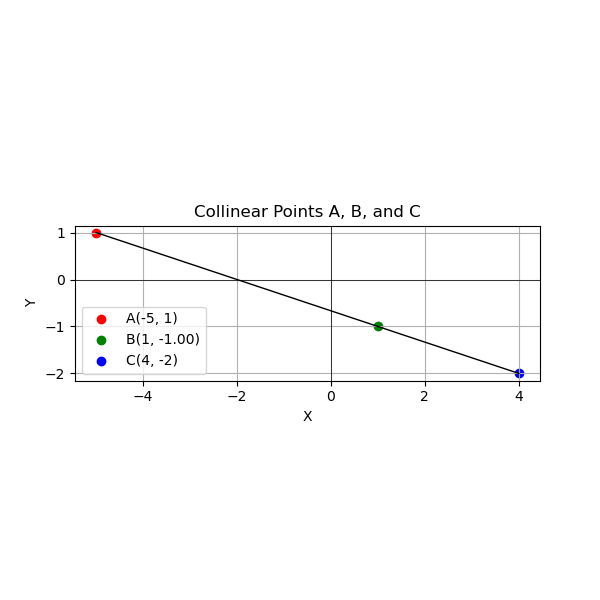
\includegraphics[width=0.7\linewidth]{figs/Figure_1.png}
 \caption{plot for collinear points}
  \label{fig. 1-1.2-18-1}
\end{figure}
\end{document}
